 % arara: xelatex: {shell: true}
% arara: biber
% arara: xelatex: {shell: true}
% arara: xelatex: {shell: true}

% Podklad k cvičení v předmětu BI-DPR
% autor: Ondřej Guth (ondrej.guth@fit.cvut.cz)
% (c) FIT ČVUT, 2018


\documentclass[a4paper]{article}
\usepackage{polyglossia}
\setmainlanguage{czech}
\usepackage{xevlna,xltxtra}
\usepackage{csquotes}
%\usepackage[style=german]{csquotes} % pro starší verze, kde není čeština

\usepackage[hidelinks]{hyperref}
\usepackage{graphicx}
\usepackage{minted}
\usemintedstyle{colorful}
\usepackage{xfrac}
\usepackage{nicefrac}
\usepackage{pdflscape}
\usepackage[style=iso-numeric]{biblatex}

\title{MI-PAA\\
\large Úkol 3 -- zpráva\\}

\author{Tomáš Přeučil}

\begin{document}

\maketitle

%\tableofcontents

%♫Playing with the queen of hearts♫
\section{Zadání úlohy}
	Zadáním úlohy bylo prozkoumání citlivosti metod řešení problému batohu na parametry instancí generovaných generátorem náhodných instancí. Na základě zjištění mělo být provedeno experimentální vyhodnocení kvality řešení a výpočetní náročnosti. Zkoumané metody měly být následující: hrubá síla, branch and bound, dynamické programování (dle ceny, nebo dle kapacity) a heuristika s poměrem cena/váha.

\section{Použité prostředky}
	\subsection{Programovací jazyky a software}
		Samotné úlohy byly řešeny v jazyce Python ve verzi 3.6 pod operačním systémem OS X 10.11.6. Program byl spouštěn z Bashe a tudíž pro spuštění nebylo využito žádné IDE.

		Pro vygenerování byl použit generátor náhodných instancí dostupný na Moodle. Pomocí tohoto generátoru bylo vygenerování 2550 různých vstupů, které jsou rozebírány dále. Skript pro generování instancí je v příloze.
		
		Pro měření času byla využita knihovna time a funkce \textit{time.process\_time()}. Jedná se o novinku od verze 3.3, která pracuje velmi podobně jako doporučovaná knihovna \textit{timeit}. Pro tuto úlohu jsou však časy relativně nepodstatné a tak jsou uvedeny pouze jako zajímavost v příloze. 
		
	\subsection{Konfigurace testovacího stroje}
		Testování bylo provedeno na MacBooku Pro 13", Early 2011, modelové číslo MC700LL/A. Stroj obsahuje CPU Intel Core i5 2415M (2,3~GHz) a 16~GB RAM. Jediný další rozdíl oproti výchozí konfiguraci je vyměněný disk (za SSD), což však v tomto případě nehraje roli.

\section{Rozbor možných variant řešení, jejich výběr a popis postupu}
	Cílem bylo měřit výpočetní náročnost a relativní chybu daných algoritmů. V případě této úlohy není vhodné měřit čas výpočtu, ale počet vnitřních stavů (jak koneckonců uvádí i zadání).
	
	Vzhledem k tomu, že hrubá síla, dynamické programování i branch and bound vrací exaktní řešení, nemá cenu u nech tento parametr testovat. Stejně tak nemá cenu testovat počet vnitřních stavů při použití heuristky -- je lineárně závislý pouze na počtu věcí v instanci.
	
	Jedním z prvních parametrů pro výběr je volba dekompozice v dynamickém programování. Zvolena byla varianta podle váhy (z důvodu velmi snadného počítání navštívených stavů).
	
	Ideálním způsobem měření je fixace všech parametrů instance a pohyb pouze jednoho. Základní nastavení generátoru proto bylo následující \mint{bash}{./a.out -I 1 -n 20 -N 50 -m 0.5 -W 100 -C 300 -k 1 -d 0} přičemž parametry pro počet věcí na instanci a počet instancí byly zafixovány v průběhu celého měření.
	
	%parametry instancí
	\subsection{Použitá data}
		Vygenerované datasety jsou následující:
		\begin{itemize}
			\item test pro poměr kapacity batohu ku sumární váze ($9*50$ instancí pro $m = 0,1...0,9$),
			\item test závislosti na maximální váze ($8*50$ instancí pro $ W =$ 50, 100, 500, 1 000, 50 000, 100 000, 500 000 a 1 000 000),
			\item test závislosti na maximální ceně ($7*50$ instancí pro $C =$ 100, 500, 1 000, 50 000, 100 000, 500 000 a 1 000 000) a
			\item test granularity pro každé i z \{-1, 0, 1\} ($3*9*50$ instancí pro $k = 0,1...0,9$).
		\end{itemize}
	
		Celkem se tedy jedná o 2 550 instancí. Skript pro generování, vygenerované instance i jejich spočtené výsledky lze najít v příloze. Stejně tak se v příloze nachází grafy z následující sekce v plném rozlišení.		

	
	\subsection{Způsob měření a následné zpracování dat}
		Pro měření byly využity funkce naprogramované v domácích úkolech 1 a 2. Data ze vstupního souboru byla načítána do pythonového skriptu, kde v každé iteraci (jedna iterace $==$ jeden řádek vstupu)	byla provedena měření na všech čtyřech algoritmech. Jak je uvedeno výše, pro každou formu problému bylo vygenerováno 50 instancí jejichž výsledky byly průměrovány.
		
		Výsledek každé iterace byl vypsán na standardní výstup a pomocí filtru tee uložen do souboru. Ten byl pomocí awk převeden na validní csv a nainportován do LibreOffice.
		
		V LibreOffice byly spočteny průměrné časy, relativní chyba, etc. Za pomocí vestavěného nástroje byly z dat vytvořeny grafy.

\section{Předpoklady, naměřené výsledky a jejich srovnání}
	\subsection{Kapacita vs. sumární hmotnost}

		Prvním experimentem bylo měření počtu stavů v závislosti poměru kapacita / sumární váha.  Předpokladem byl lineární růst pro DP (roste kapacita, tudíž i počet nutných průchodů), což se potvrdilo.
	
		U branch and bound počet stavů nejprve roste a pak klesá. Nejspíše je to způsobeno efektivním prořezáváním (najdeme předmět, co překračuje kapacitu a zařízneme větev). V momentě průměrného poměru pak dává smysl vyšší výpočetní náročnost.
	
		Implementovaná hrubá síla není úplně primitivní a funguje zde zaříznutí větve po přesažení kapacity batohu a z toho důvodu do jisté míry kopíruje průběh BaB pro nízké poměry (implementace vychází z prvního úkolu). Dále pak ale není citlivá vůbec na nic.	
		
		Vše je reprezentováno na grafu \ref{states-capVsWeight}.
	
		\begin{figure}[h]\centering
			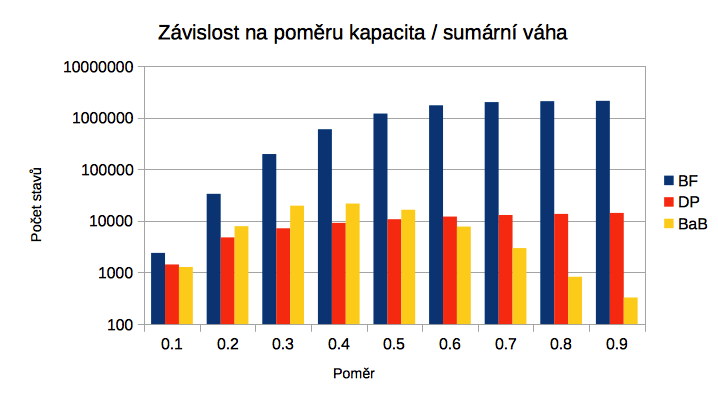
\includegraphics[width=0.99\textwidth]{states-capVsWeight.png} 
			\caption{Závislost na poměru kapacita / sumární váha}
			\label{states-capVsWeight}
		\end{figure}
	
		Pro heuristiku byla měřena přesnost. Je nutné poznamenat, že ta byla až překvapivě vysoká. Na grafu \ref{err-capVsWeight} lze vidět snižující se tendenci chyby pro zvyšující se koeficient.

		\begin{figure}[h]\centering
			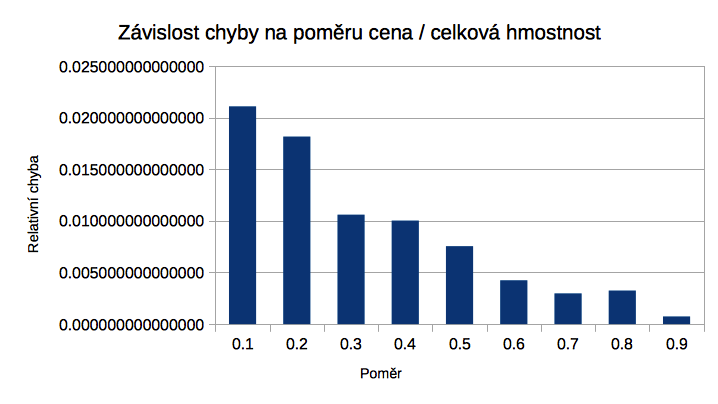
\includegraphics[width=0.99\textwidth]{err-capVsWeight.png} 
			\caption{Závislost chyby na poměru cena / sumární hmotnost}
			\label{err-capVsWeight}
		\end{figure}
	
	\subsection{Maximální cena}
	
		Další měřenou veličinou byla závislost výpočetní složitosti na maximální ceně věcí. Hrubá síla byla nepřekvapivě necitlivá na libovolný pohyb.
	
		Totéž lze ale říci i o dynamickém programování (byla použita dekompozice dle kapacity, takže se nejedná o překvapivé zjištění), ale i o branch and bound, kde byl však počet navštívených stavů přibližně 2x vyšší.
	
		Reprezentace dat se nachází na grafu \ref{states-maxValue}.
		
		\begin{figure}[h]\centering
			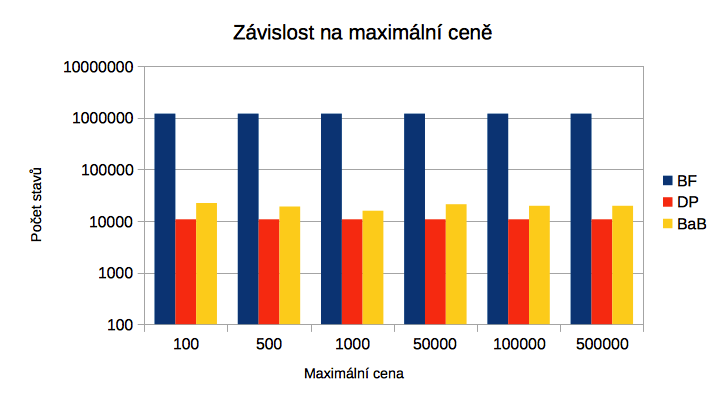
\includegraphics[width=0.99\textwidth]{states-maxValue.png} 
			\caption{Závislost na maximální ceně}
			\label{states-maxValue}
		\end{figure}
		
		Co se týče heuristiky, z naměřených dat lze říci, že relativní chyba na maximální ceně nezávisí -- vizte graf \ref{err-maxValue}.
	
		\begin{figure}[h]\centering
			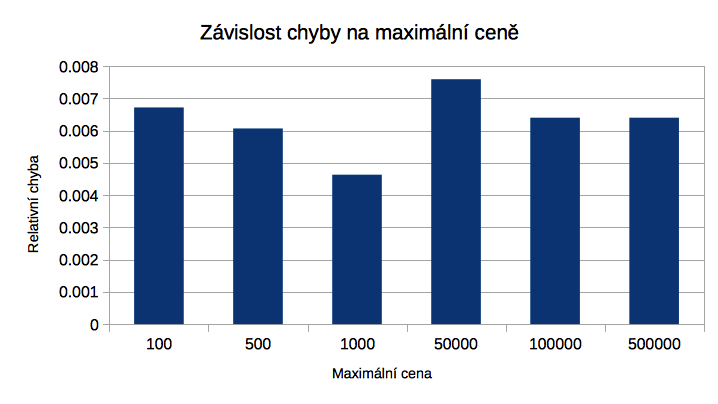
\includegraphics[width=0.99\textwidth]{err-maxValue.png} 
			\caption{Závislost chyby na maximální ceně}
			\label{err-maxValue}
		\end{figure}
	
	\subsection{Maximální váha}
	
		Třetím experimentem bylo měření závislosti na maximální váze. Hrubá síla byla, opět, nepřekvapivě zcela necitlivá.
		
		Počet navštívených stavů u dynamického programování roste víceméně lineárně, což vzhledem k použití dekompozice dle kapacity dává smysl. Musíme navštívit mnohem více stavů.
		
		Jako nejefektivnější pro váhu 500 a vyšší se ukázala metoda branch and bound, jejíž složitost sice mírně roste (pro cenu 50 a 100 000 je rozdíl cca 1,5násobný), ale i přesto jasně překonává všechny ostatní exaktní metody.
		
		Data jsou na grafu \ref{state-maxWeight}.
		
		\begin{figure}[h]\centering
			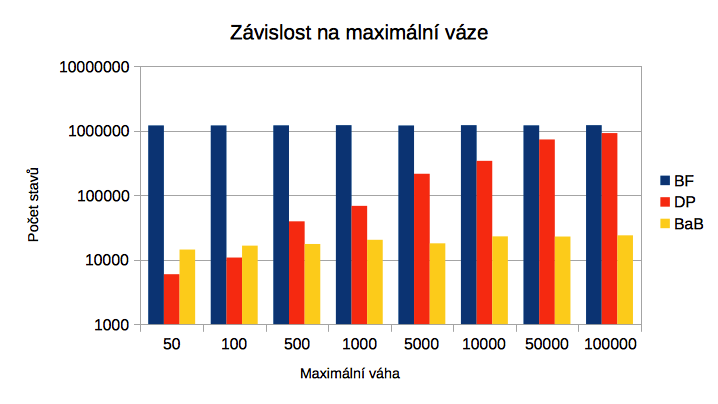
\includegraphics[width=0.99\textwidth]{states-maxWeight.png} 
			\caption{Závislost na maximální váze}
			\label{state-maxWeight}
		\end{figure}
		
		Dle provedeného měření je relativní chyba heuristiky na maximální cenu necitlivá, což dokazuje i graf \ref{err-maxWeight}.
	
		\begin{figure}[h]\centering
			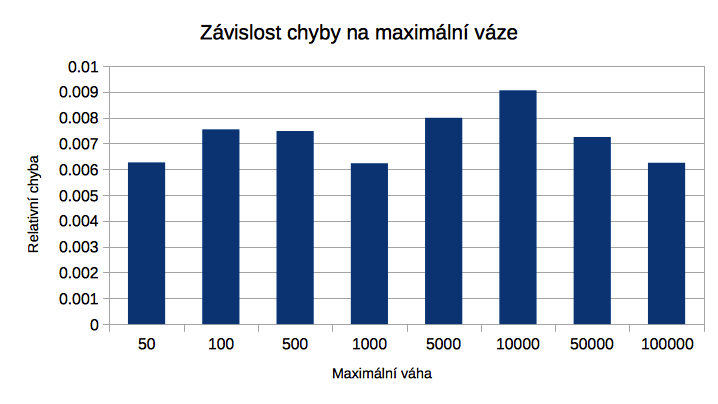
\includegraphics[width=0.99\textwidth]{err-maxWeight.png} 
			\caption{Závislost chyby na maximální váze}
			\label{err-maxWeight}
		\end{figure}
		

	\subsection{Granularita}
	
		Posledním experimentem bylo celkem 27 (krát padesát instancí) měření pro granularitu. Zde byly provedeny experimenty pro všechny tři možné hodnoty d (-1 -- více malých věcí, 1 -- více velkých věcí, 0 -- rovnováha) byly zkoumány hodnoty k od 0,1 do 0,9.
		
		I zde se hrubá síla ukázala jako necitlivá. To byl jediný předpoklad před měřením.
		
		Dynamické programování ukázalo citlivost na exponent v momentě, kdy nebyla zvolena rovnováha. Vyhovují mu tedy spíše malé věci. Branch and bound algoritmus se choval obdobně, ve většině případů však navštívil výrazně více stavů. Vše je vidět na grafu \ref{states-granularity}.
		
		O citlivosti heuristiky lze říci jen to, že čím větší je v instanci rovnováha, tím konzistentnější bude relativní chyba. Více se ze změřených dat poznat nedá, jak ukazuje graf \ref{err-granularity}.
		
		
\section{Závěr}
	Byla provedena analýza dříve implementovaných algoritmů na více než 2 500 různých instancích. Byla prokázána domněnka, že hrubá síla je necitlivá na vstupní data (s jednou výjimkou danou implementací).
	
	Dále byly porovnány další algoritmy (branch and bound, dynamické programování s dekompozicí podle váhy a heuristika s poměrem cena/váha). Výsledkem je možnost výběru použitého algoritmu pro exaktní řešení, pokud předem známe některý z parametrů.
	
	Z hlediska heuristiky byla prokázána korelace relativní chyby na poměru ceny a sumární hmotnosti, ostatní korelace se prokázat nepodařilo. Jedná se však o velmi rychlý algoritmus jehož počet kroků záleží pouze na velikosti instance.

		\begin{landscape}
			\begin{figure}[h]\centering
				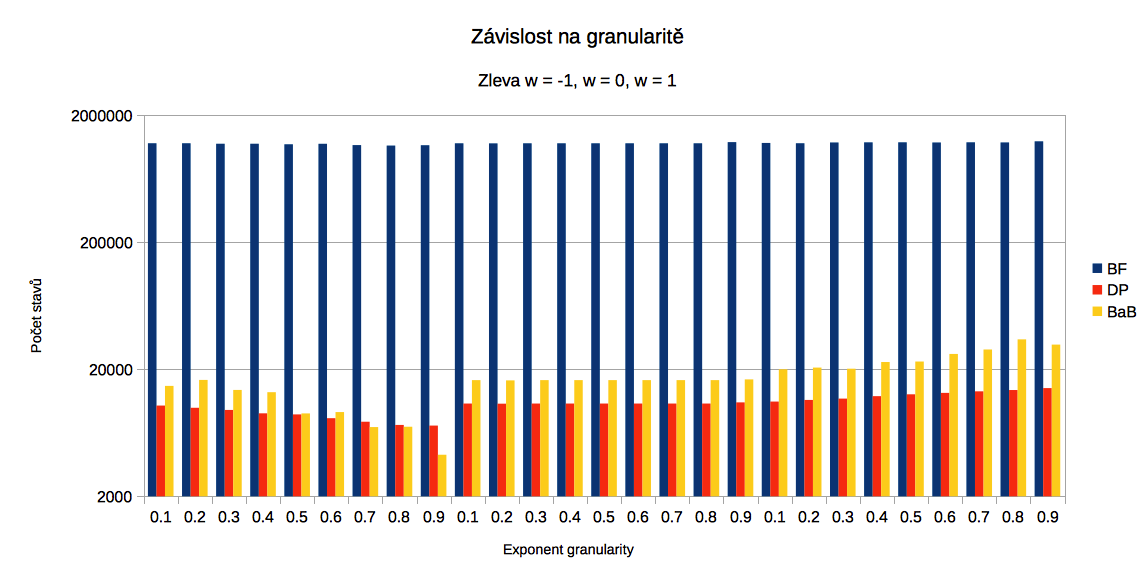
\includegraphics[height=0.94\textwidth]{states-granularity.png} 
				\caption{Závislost na granularitě}
				\label{states-granularity}
			\end{figure}

			\begin{figure}[h]\centering
				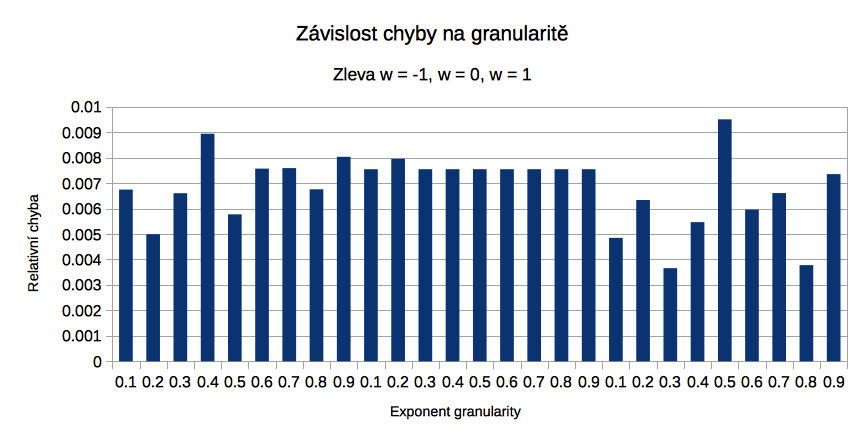
\includegraphics[height=0.94\textwidth]{err-granularity.png} 
				\caption{Závislost chyby na granularitě}
				\label{err-granularity}
			\end{figure}
		\end{landscape}
		
\end{document}